\Subsection{Definitions}

\begin{definition}\textbf{Graph}
    Graph $G$ is a pair of sets: the set of verticies $V$ and the set of edges $E$ represented as a set of pairs of verticies, $G := (V,\ E)$.
\end{definition}

\begin{definition}\textbf{Basics}

    1. If edges have directions then the graph is called \textbf{directed graph}.

    2. If edges do not have any directions then the graph is called \textbf{undirected graph}.

    3. If each edge has a corresponding weight assigned to it then the graph is called \textbf{weighted graph}.

    4. If $E$ is a \textit{multiset}, i.e. some verticies may have several edges between them, then such edges are called \textbf{multiple edges} and the graph may be called \textbf{multi-gprah}.

    5. For an edge $e = (a,\ b)$ we say that $e$ is \textbf{incident} to the vertex $a$/$b$.

    6. The \textbf{degree} of a vertex is the number of its incident edges, denoted as $\deg{v}$.

    7. In the directed graph there are \textbf{incoming} and \textbf{outgoing} degrees: $\deg{v} = \deg_{in}{v} + \deg_{out}{v}$.

    8. Two edges that share a common vertex are called \textbf{adjacent} edges.

    9. Two verticies that are connected by an edge are also called \textbf{adjacent}.

    10. If $\deg{v} = 0$ then $v$ is an \textbf{isolated} vertex.

    11. If $\deg{v} = 1$ then $v$ is a \textbf{leaf} in a graph.

    12. An edge $e = (v,\ v)$ is called a \textbf{loop}.

    13. A \textbf{simple graph} is a graph that does not have more than one edge between any two vertices and no edge starts and ends at the same vertex (i.e. no multi-edges and no loops).

\end{definition}

\begin{definition}\textbf{Path}

    A path in a graph is an alternating sequence of vertices and edges in which neighboring elements are incident and the extreme ones are vertices. In the digraph, the direction of all edges is from \textbf{i} to \textbf{i+1}.

    E.g., $v_0 \to e_0 \to v_1 \to e_1 \to v_2 \to e_2 \to v_3 \to ... \to e_{k-1} \to v_k$.

\end{definition}

\begin{definition}

    1. The path is \textbf{vertex simple/simple} if all its verticies are distinct.

    2. The path is \textbf{edge simple} if all its edges are distinct.

    \underline{Note}: paths exist in both undirected and directed graphs; if there are no multi-edges in the graph then each path can be denoted merely via its verticies.

    3. \textbf{Cycle} is a path with equal extreme verticies (i.e. both the start and the end are the same vertex).

    4. Cycles also can be \textbf{vertex simple} and \textbf{edge simple}.

    5. \textbf{Acyclic} graph is a graph with no cycles in there.

    6. \textbf{Tree} is an acyclic undirected graph.

\end{definition}


\Subsection{How to store a gprah programmically}

We will assume that $|V| = n$ and $|E| = m$. Sometimes $V$ and $E$ could be used to denote their sizes.

\Subsubsection{List of edges}

Here we merely store the vector of edges, i.e. pairs of vertex $(a_i,\ b_i)$ which denote an edge $e_i:= a_i \to b_i$:

\begin{lstlisting}[language=C++]
pair<int, int> edges[m];
// Or:
vector<pair<int, int>> edges(m);
// Or (if we want to store weights on edges):
struct Edge {int from, to, weight; };
vector<Edge> edges(m);
\end{lstlisting}

\Subsubsection{Adjacency matrix}

For each pair of vertices we can store either the fact of having/not having an edge between them (i.e. $0$ or $1$), or the number of edges between them, or the weight of an edge between them.

\begin{lstlisting}[language=C++]
bool c[n][n];
// c[a][b] = 0/1 - denotes whether vertices a and b have an edge between them
int c[n][n]; // here c[a][b] denote the weight of an edge between a and b
\end{lstlisting}

\Subsubsection{Adjacency Lists}

For each vertex $v$ we store a list of its adjacent edges:

1. $v_0 \to e_{i_0}, e_{i_1}, ..., e_{i_k}$

2. $v_1 \to e_{j_0}, e_{j_1}, ..., e_{j_p}$

...

3. $v_{n-1} \to e_{t_0}, e_{t_1}, ..., e_{t_q}$

\begin{lstlisting}[language=C++]
// to make it remove/find fast replace vector with set/unordered_set
vector<Edge> c[n];
\end{lstlisting}

\Subsubsection{Required actions with a graph}

1. \textbf{adjacent(v)} - traverse all incident edges of $v$.

2. \textbf{get(a, b)} - check the existence/weight of an edge between $a$ and $b$.

3. \textbf{all()} - check all the edges of the graph.

4. \textbf{add(a, b)} - add an edge $a \to b$.

5. \textbf{del(a, b)} - remove an edge $a \to b$.

Here are the time complexities of the operations for the described storing methods:

\begin{center}
    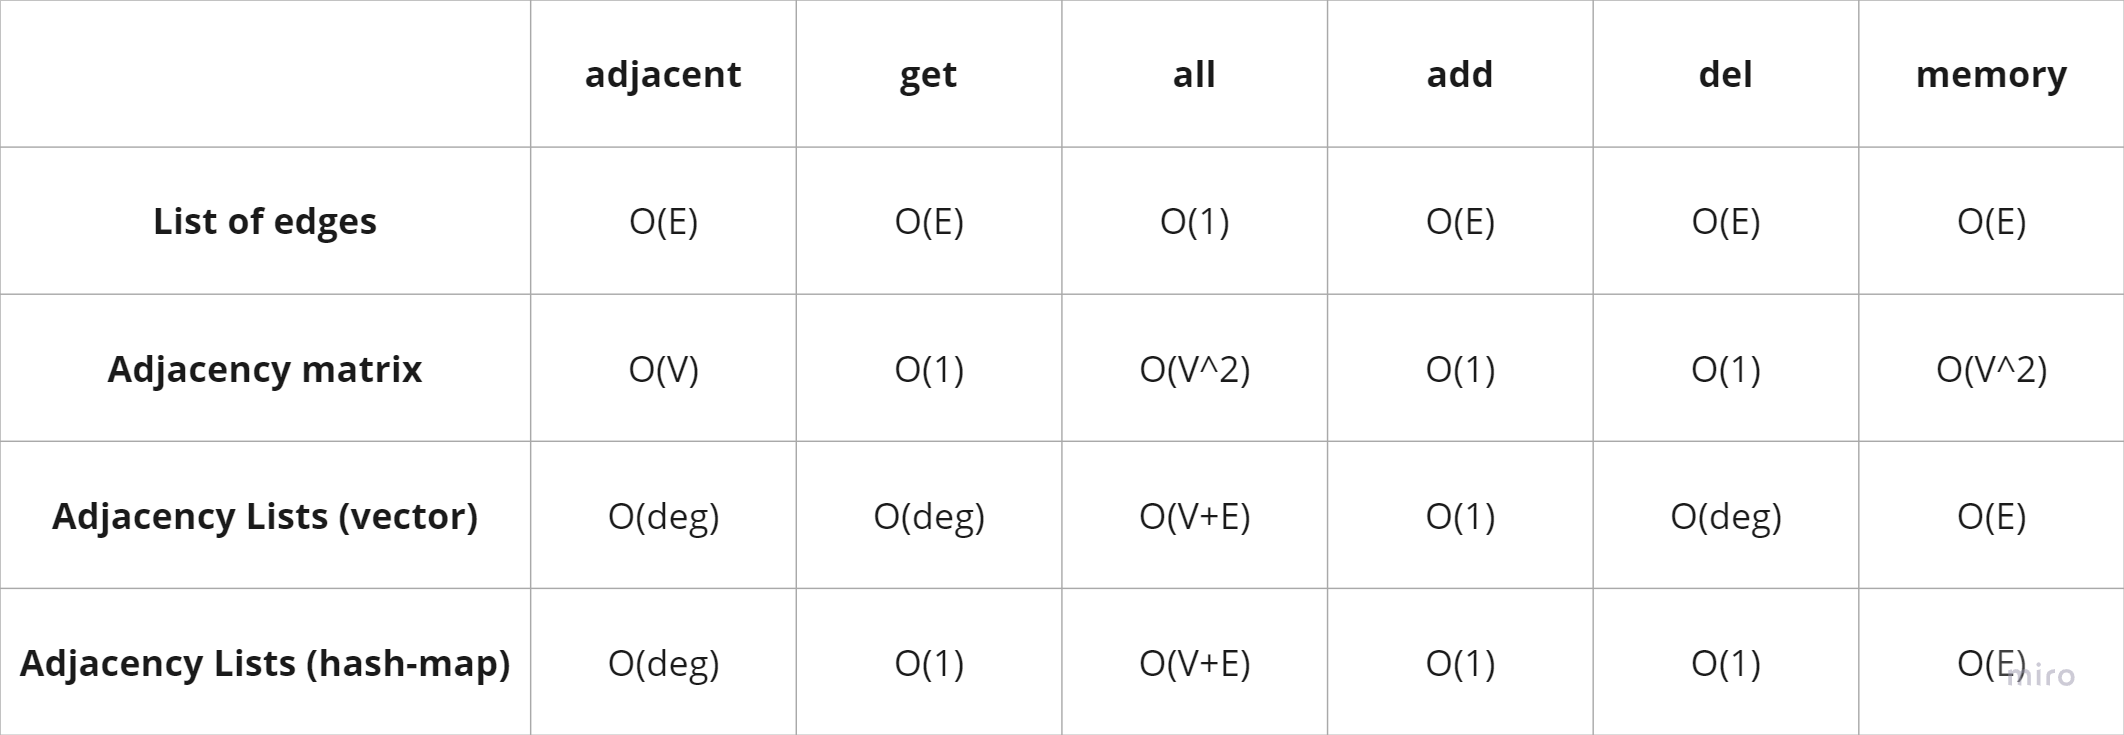
\includegraphics[scale=0.25]{./assets/14-graphs-and-basic-dfs/1.png}
\end{center}


\Subsection{dfs: depth-first search}

\textbf{Task}: mark all the vertices reachable from a given vertex $a$.

\textbf{Solution}: mark the adjacent verticies of the $a$ and then call the procedure recursively.

\begin{lstlisting}[language=C++]
vector<vector<int>> graph(n);
void dfs(int v) {
    // no need to traverse already visited verticies
    if(marked[v]) return;
    marked[v] = 1;
    for (int u : graph[v]) {
        dfs(u);
    }
}
dfs(a);
\end{lstlisting}

The time complexity is $O(E)$ because each edge is visited not more then once.

\begin{definition}\textbf{Connectivity components}
    Two verticies $a$ and $b$ are located in a single connectivity component iff $\exists$ a path between them.

    In other words, a connectivity component is a equvalence class over a relation of reachableness (i.e. $a, b \in C \leftrightarrow \exists p - \text{path}\ a \to_{p} b$).
\end{definition}

\begin{center}
    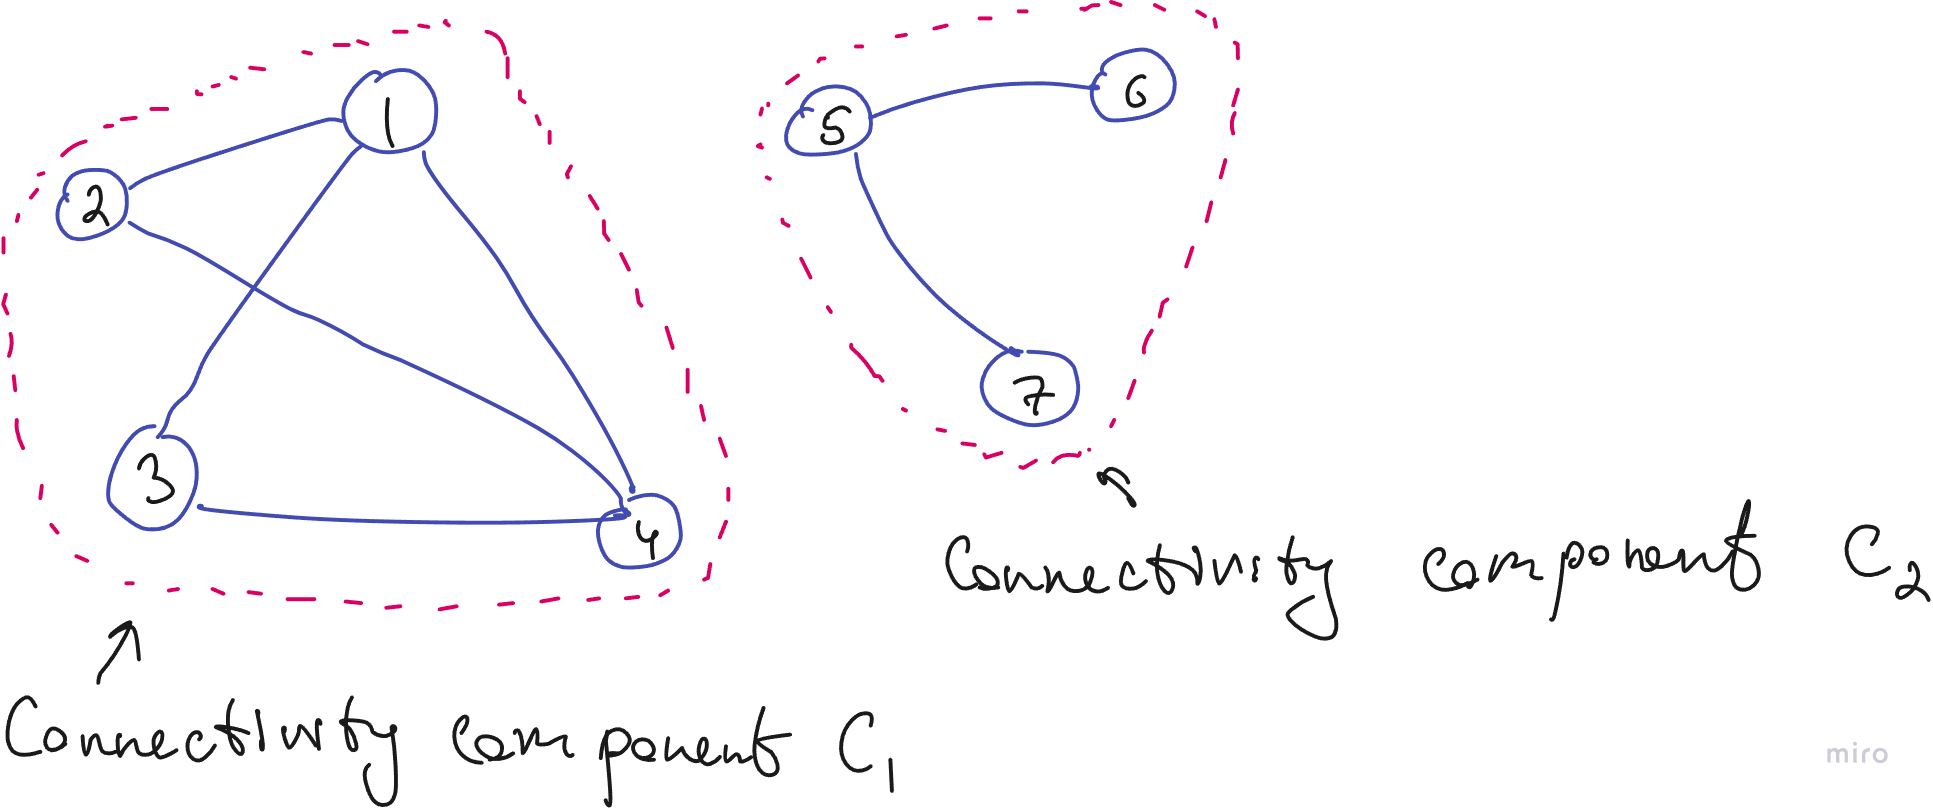
\includegraphics[scale=0.25]{./assets/14-graphs-and-basic-dfs/2.png}
\end{center}

All connectivity components may be easily found via dfs. We need to start the dfs from a vertex $v$ and it will cover all the verticies that are reachable from $v$, i.e. it will be a connectivity component.

\begin{lstlisting}[language=C++]
vector<vector<int>> graph(n);
int connectivity_component = 0;

void dfs(int v) {
    if(marked[v] != 0) return;
    marked[v] = connectivity_component;
    for (int u : graph[v]) {
        dfs(u);
    }
}

for (int v = 0; v < n; ++v) {
    if (!marked[v]) {
        connectivity_component++;
        dfs(v);
    }
}
\end{lstlisting}

Now each vertex is \textit{colored} in the color of its connectivity component. The time complexity is $O(V + E)$ because each edge is traversed only once and we traverse each vertex in the for-loop.

\Subsubsection{Path recovery}

We need to find a path from a vertex $v$ to the vertex $u$ and print the found path (assume it exists). We can collected the visited verticies as follows:

\begin{lstlisting}[language=C++]
vector<int> path;

bool dfs(int v) {
    if (v == u) {
        path.push_back(v);
        return 1 /*path found*/;
    }
    marked[v] = 1;
    for (int x : graph[v]) {
        if (dfs(x) /*x is lying on the path*/) {
            // v -> .. -> x -> .. -> u  =>  x must in added to the path
            path.push_back(x);
            return 1 /*path found*/;
        }
    }
    return 0 /*path not found*/;
}
\end{lstlisting}

Now the \textbf{path} vector contains the verticies from the $u$ to the $v$ (i.e. the order is reversed since $u$ was added first).


\Subsection{Topological sorting}

\begin{definition}
    \textbf{Topological sorting} is an ordering of the verticies of \textbf{directed} (oriented) graph according to the partial order given by the graph's edges.

    In order words, topological sorting is a mapping of integers to the verticies $a_v$, so that: $\forall e := \ v \to u: \ a_v < a_u$.
\end{definition}

\begin{lemma}
    Topological sorting exists $\leftrightarrow$ the graph is \textit{acyclic}.
\end{lemma}

\begin{proof}

    1. \textbf{$\bar{A} \leftarrow \bar{B}$}: If there is a cycle $v_1 \to v_2 \to .. \to v_{k-1} \to v_k \to v_1$, then we have the sequence of inequalities:

    $a_{v_1} < a_{v_2} < a_{v_3} < .. < a_{v_{k-1}} < a_{v_k} < a_{v_1}$ $\implies a_{v_1} < a_{v_1}$ which is false.

    2. \textbf{$A \leftarrow B$}: If there are no cycles in the graph then there exists a vertex $v$ whose $\deg_{in}(v) = 0$, then let's assign $a_{v} := 0$ and remove the vertex. There still will be no cycles, do the same procedure until no verticies left in the graph $\implies$ topological sorting is constructed.

\end{proof}

\begin{lstlisting}[language=C++]
// non-recursive solution
vector<int> topSort(vector<vector<int>>& graph /*directed graph*/) {
    vector<int> ans;
    int start = find_vertex_of_zero_indeg(graph); // assert it exists

    queue<int> q = { start };
    while (!q.empty()) {
        int v = q.front(); q.pop();
        ans.push_back(v);
        // we remove vertex v and update indegs of its neighbors
        for (int u : graph[v]) {
            if (--deg[u] == 0) {
                q.push(u);
            }
        }
    }

    return ans;
}

// recursive solution
vector<int> ans;
void dfs(int v) {
    if (marked[v]) return;
    marked[v] = 1;
    for (int u : graph[v]) {
        dfs(u);
    }
    ans.push_back(v);
}
std::reverse(std::begin(ans), std::end(ans));
for (int v : ans) {
    std::cout << v << " ";
}
\end{lstlisting}
